% !TeX root = ../../main.tex
\section{Mechanical design}
\subsection{Material selection}
The strong oxidising nature of nitric acid as a result of autocatalytic reduction gives nitric acid a very corrosive property of \SI{70}{\percent\wv} \cite{suresh_corrosion_nodate}. The reactor material needs to be carefully selected to ensure the reactants do not corrode the walls, which gives rise to more possible locations for a hotspot to develop. Several stainless steel have been shortlisted for selection: 1) Stainless steel Type 304, 2) Stainless stell Type 316, and 3) Stainless steel Type 304L
%\begin{enumerate}
    %\item Stainless steel Type 304
    %item Stainless steel Type 316
    \item Stainless steel Type 304L
%\end{enumerate}

Stainless steel Type 304 has a higher level of carbon not stabilised with titanium or niobium. This makes it susceptible to intergranular attack from nitric acid at heat-affected zones of the welds. Chromium carbides precipitate at the grain boundaries \cite{cm_selection_nodate}, which causes the oxidation of the protective chromium passive film and reducing the material's corrosion resistance. Stainless steel Type 316 includes molybdenum additions which are generally known to improve resistance to acid corrosion, but in the case with nitric acid, molybdenum tends to promote the formation of a sigma phase, which is known to cause extreme reduction in corrosion resistance. Thus, stainless steel type 304L (also identified as BS EN 10088-1.4307) was selected for both the reactor tube and shell as it is a low-carbon, stabilised stainless steel which has excellent corrosion resistance due to its chromium passive film \cite{ningshen_corrosion_2011}.

%-chosen material to be stainless steel 304L based on paper
\subsection{Design pressure and temperature}
\subsubsection{Reactor tube}
\cref{sec:adiabatic} requires the reactor to operate below \SI{363}{\K} and a pressure gradient of \SIrange{1}{1.3}{\bar}. The design temperature is set as \SI{363}{\K} following the maximum operating temperature and design pressure ($p_d$) is calculated to be \SI{1.44}{\bar}, using \cref{eqn:designpressure} below:
\begin{equation}
    p_d = \frac{P_o}{0.9} = \frac{1.3}{0.9} = \SI{1.44}{\bar}
    \label{eqn:designpressure}
\end{equation}

\subsubsection{Shell}
Similarly, using \cref{eqn:designpressure}, $p_d$ for the cooling water vessel was calculated to be \SI{1.1}{\bar} from an operating pressure ($p_o$) of \SI{1}{\bar}. The design temperature for the cooling water vessel is set as \SI{328}{\K}, as it is the upper bound of the ambient temperature range of the cooling water stream. 

\subsection{Reactor dimension design}
\label{sec:reactordimensions}

\subsubsection{Reactor tube dimensions}
\label{sec:reactortube}
From \cref{sec:detailedreactor}, the total flowrate across the entire reactor was calculated to be \SI{1.32e-4}{\cubic\m\per\s}. Dividing by the number of tubes calculated from \cref{eqn: hexagon}, gives the flowrate across one individual tube as \SI{1.88e-5}{\cubic\m\per\s}. An optimal length of \SI{4.3}{\metre} and a final diameter for the reactor tubes of \SI{230}{\milli \metre} were set as previously determined in \cref{sec:coolanttemp,sec:axialdispersion}. 

The minimum thickness of the reactor tubes ($e_\mathrm{reactor}$) was calculated using \cref{eqn:minthicknessreactor},
\begin{equation}
    e_\mathrm{reactor} = \frac{p_dD_i}{2f-p_d} = \frac{0.14 \times 230}{2 \times 111 - 0.14} = \SI{0.145}{\mm}
    \label{eqn:minthicknessreactor}
\end{equation}
where inner reactor diameter ($D_i$) is defined as \SI{0.23}{\metre} from \cref{sec:axialdispersion}, design pressure ($p_d$) is calculated to be \SI{1.44}{\bar}, nominal design stress ($f$) is defined \SI{111}{\N\per\square\mm} for design temperature not exceeding \SI{423}{\K} based on BS5500 standards , yield stress ($\delta_y$) is defined as \SI{215}{\N\per\square\mm} \cite{noauthor_unfired_nodate}.


\begin{wrapfigure}{r}{0.4\linewidth}
    \centering
    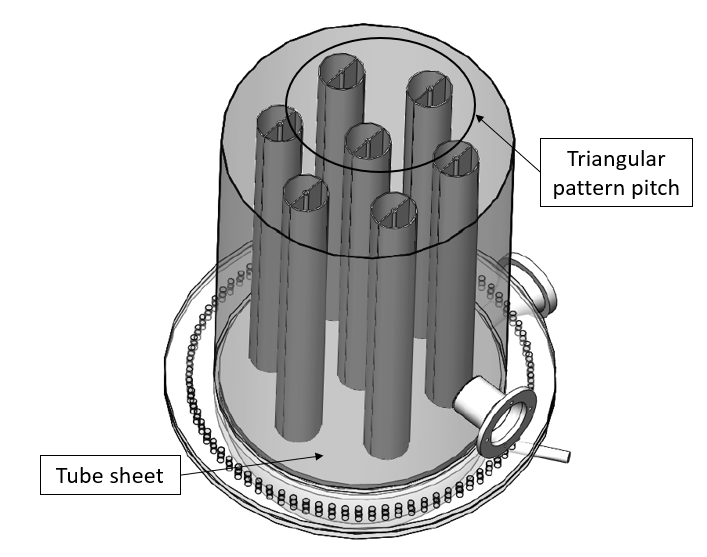
\includegraphics[width=\linewidth]{chapters/2-reaction/figures/FYD 7tube cross section with label.PNG}
    \caption{3D cross section of reactor tube arrangement}
    \label{fig:reactortubearrangement}
\end{wrapfigure}
7 tubes were selected as the optimal number based on the centered hexagonal number rule (see \cref{eqn: hexagon}) which has widespread usage in industry for maximising the number of tube bundles in large cylindrical containers \cite{noauthor_realiable_2018}. 
\begin{equation}
    n^3 - (n-1)^3 = 3n(n-1)+1
    \label{eqn: hexagon}
\end{equation}
where $n$ represents the sequence of hexagonal number. 

The tube bundle was arranged to give a clearance of \SI{230}{\milli \metre}, which satisfies the minimum clearance of 0.25 times the tube diameter to maximise the cooling heat transfer coefficient, according to Primo et al \cite{primo_shell_2012} . 2 tube sheets were fitted at each end of the shell to secure the tubes in position. A triangular pattern pitch layout was selected to complement the hexagonal tube arrangement and to offer a more robust tube sheet construction \cite{primo_shell_2012}. The arrangement of 7 tubes held by the tube sheet is shown in \cref{fig:reactortubearrangement}.

\subsubsection{Secondary cooling tube dimensions}
As mentioned in \cref{sec:tripleconctube}, the secondary cooling water system was implemented in a triple concentric tube (TCTHE) manner within the reactor tubes to prevent thermal runaway and hotspots. Each secondary cooling water tube was designed to have a diameter of \SI{20}{\milli \metre} with a flowrate of \SI{2.1e-4}{\cubic\m\per\s}. The wall thickness was also set as \SI{5}{\milli \metre} for a standardised production with the shell and head vessel. 
The arrangement of the secondary cooling tube within the reactor tubes can be visualised in the cross section shown in \cref{fig:concentriccoolingwater}. 
\begin{figure}[H]
    \centering
    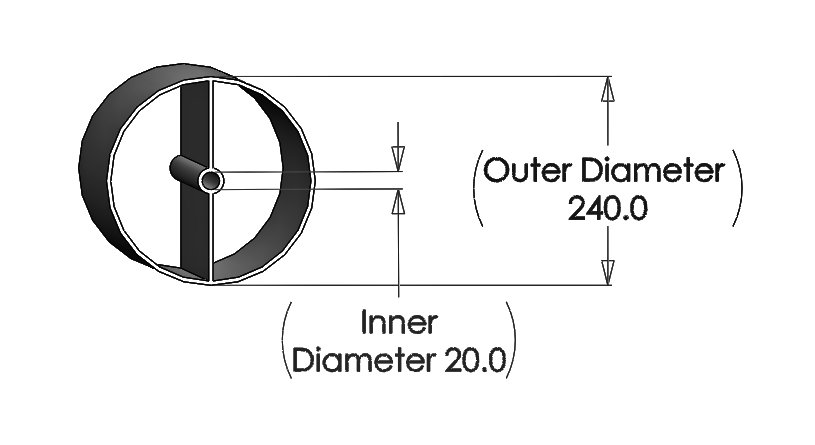
\includegraphics[width=0.5\linewidth]{chapters/2-reaction/figures/FYD conc tube with calc bw.png} 
    \caption{3D cross section of concentric secondary cooling water system}
    \label{fig:concentriccoolingwater}
\end{figure}

\subsubsection{Shell dimensions}
The diameter of the shell was \SI{1.5}{\metre} to withstand a total cooling water mass flowrate of \SI{2.3}{\kilogram \per \second}.
Similarly, the minimum thickness of the shell ($e_\mathrm{shell}$) was calculated using equation \cref{eqn:minthicknessreactor}, where $D_i$ set as \SI{1500}{\milli \metre}, $p_d$ as 0.11 and $f$ value of \SI{143}{\N\per\square\mm}. The minimum thickness of the shell was calculated to be \SI{0.577}{\milli \metre}. After taking into account corrosion allowance of \SI{1.5}{\milli \metre} and other welding considerations, a final shell thickness of \SI{5}{\milli \metre} was chosen. 

\subsubsection{Head dimensions}
%A torispherical head was chosen as the preferred over ellipsoidal and hemispherical heads due to higher maximum stress and deformation threshold (). 
A hemispherical head was chosen as the preferred head as the pressure in the vessel is divided equally across the surface of the head, making it suitable for large sized pressure vessels. The minimum thickness ($e_\mathrm{head}$) of the hemispherical head was calculated using \cref{eqn:hemisphericalend},
\begin{equation}
    e_\mathrm{head} = \frac{pD_i}{2f-0.2p} = \frac{0.14 \times 1500}{2 \times 143 - 0.2 \times 0.14} = \SI{0.73}{\mm}
    \label{eqn:hemisphericalend}
\end{equation}
with $p$ set as \SI{1.4}{\bar}, $D_i$ set as \SI{1500}{\milli \metre}, $f$ value set as \SI{143}{\N\per\square\mm}.  The minimum thickness of the hemispherical end was calculated to be \SI{0.73}{\milli \metre}, but a final head thickness of \SI{5}{\milli \metre} was chosen to complement the thickness of the shell for ease of welding. 
%-refer BS5500 page 78 of the pdf

The minimum distance ($L_{im}$) between ports were calculated using \cref{eqn:mindistance} below,
\begin{equation}
    L_m = \sqrt{(2r_{im}+e_{m})e_m} = \sqrt{(2 \times 1500 + 5)5} = \SI{122.6}{\mm}
    \label{eqn:mindistance}
\end{equation}
where $r_{im}$ denotes the radius of inner diameter and $e_m$ denotes the thickness of the shell. The minimum distance between ports on the dome was calculated to be \SI{122.6}{\milli \metre} apart. 

%-label and explain this equation
%rewrite based on hemispherical
\subsection{Ports and flanges design}
A total of 7 ports were designed according to the BS 5500:1997 and BS 1600:1991 standards for the inlet and outlet of reactants, primary and secondary cooling water, and a pressure relief valve (PRV). Based on BS1600: 1991, schedule 40 pipes were chosen for all pipes \cite{noauthor_dimensions_nodate}. 
%inlet and outlet ports for feed reactants, and one pressure relief valve (PRV). 

\subsubsection{Reactant flow port design} \label{sec:reactantport}
The reactant inlet and outlet flows were placed at the top right and top left of the hemispherical shell domes respectively. Both ports were estimated to have an acceptable feed liquid velocity range (U) of \SIrange{0.1}{1}{\m\per\s}. The cross sectional area (A) is then calculated by dividing the volumetric flowrate ($Q_v$) by the liquid velocity. $Q_v$ is determined as \SI{9.24e-4}{\cubic\m\per\s} and a first approximation of \SI{0.1}{\m\per\s} for the liquid velocity led to an initial port diameter of \SI{108.5}{\milli \metre}. Based on BS 1600:1991, with a \SI{6}{\milli \metre} wall thickness, the minimum outer diameter (OD) of the reactant inlet and outlet ports was chosen to be \SI{114.3}{\milli \metre} (4" NPS). 

\subsubsection{Cooling water flow port design}
Similarly, the outer pipe diameter of both the primary and secondary cooling water flow ports were calculated as previously described in section \ref{sec:reactantport}. The primary cooling water port was defined to have an OD of \SI{219.1}{\milli \metre} (8" NPS) with \SI{6.55}{\milli \metre} of wall thickness, whereas the secondary cooling tube had an OD of \SI{60}{\milli \metre} (2" NPS) with \SI{4}{\milli \metre} of wall thickness. All port dimensions were calculated based on information from BS 1600:1991. 

\subsubsection{Pressure relief valve design}
A PRV was included as a safety device to protect the vessel and relief pressure in case of a overpressure event. An overpressure event will occur when the pressure is beyond the design pressure (also known as maximum allowable working pressure, MAWP) \cite{marsha_lecture_nodate}. Detailed calculation based on API 250 standard of the sizing of safety relief valves for liquid can be viewed in \ref{app:PRV} \cite{api_standard_520_sizing_2013}.

Due to the highly flammable nature of the nitration reaction, the maximum allowable accumulated pressure was designed for fire exposure at 1.21 times the maximum allowable working pressure (MAWP), which is then calculated to be \SI{1.74}{\bar}. The final PRV size for schedule 40 steel was calculated to have an OD of \SI{101.6}{\milli \metre} (3 $\frac{1}{2}$" NPS) and a wall thickness of \SI{5.74}{\milli \metre}.
%- Inlet of water on top, outlet of water at the bottom. Size the water

%what is the arramgement of the piping? are we looking at all 19 stacked into one huge tube of diameter 100+cm? 


\subsubsection{Flange types and dimension}
Class 150 flanges were chosen from Table 16 of BS 1560:1989 \cite{noauthor_circular_nodate}, based on the maximum permissible working pressure and temperature, which provided a suitable pressure temperature rating for the stainless steel type 304L (material group 2.3). Weld-neck flanges were selected for all ports due to their high structural strength along with good stress distribution \cite{ulma_forge_welding_2020}.
Based on the JPI 75-48-73 standard, the nominal pipe size (NPS) for the flanges was selected as 54" for class 150 flanges.

\subsubsection{Gasket type and dimension}
A gasket is a sealing material placed between flanges to create a leak-proof sealing \cite{varun_piping_nodate}. A narrow-faced, ring joint gasket type was chosen due to the suitability of design when corrosive agents are present \cite{noauthor_ring_nodate}. The octagonal soft steel gasket was chosen to complement a ring joint gasket as it is softer than the flange material, to ensure sufficient deformation of the gasket without damaging the flange facing. The chosen gasket has a gasket factor (m) of 5.5 and minimum design seating stress (y) of \SI{124}{\N\per\mm} \cite{noauthor_unfired_nodate}.

\subsubsection{Bolt types and dimension}
The bolting material was selected as mild and carbon steel (BS 3692 grade 8.8), which is capable of withstanding the \SI{174}{\N\per\square\mm} design stress and for temperatures not exceeding \SI{100}{\celsius}. Based on the JPI 7S-48-73 standard for large diameter flanges, the diameter of the bolt circle was defined as \SI{1492}{\milli \metre}, with 56 bolts each of \SI{32}{\milli \metre} diameter for 54" NPS flanges. 

\subsection{Overall design}
The overall cross sectional design of the reactor can be seen in \cref{fig:mainreactor} below. Additional mechanical design drawings from SolidWorks are included in \cref{app:engineeringdesign}.
\begin{figure}[h]
    \centering
    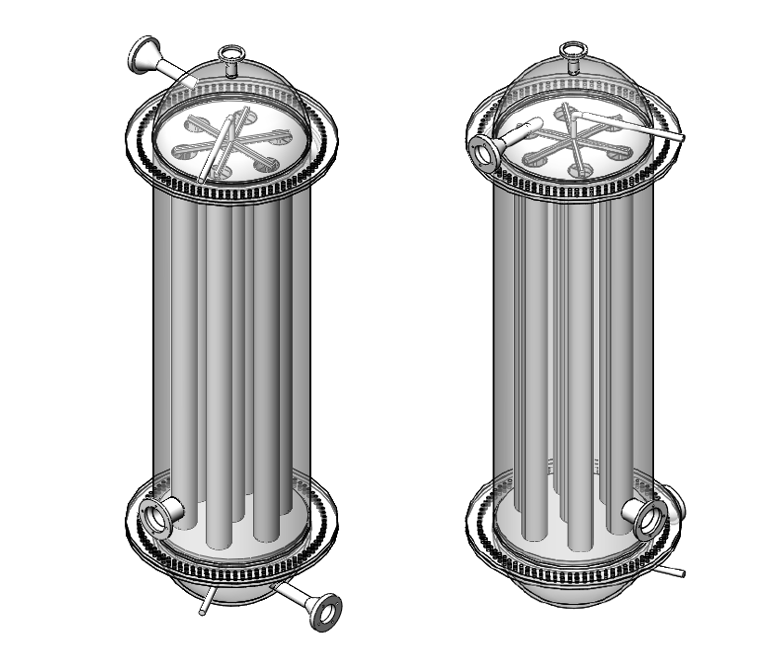
\includegraphics[width=0.6\linewidth, scale=0.5]{chapters/2-reaction/figures/FYD reactor poster boy both.PNG}
    \caption{Overall design of HEX reactor}
    \label{fig:mainreactor}
\end{figure}

